\documentclass[tikz,border=4pt]{standalone}
\usepackage{amsmath}
\begin{document}
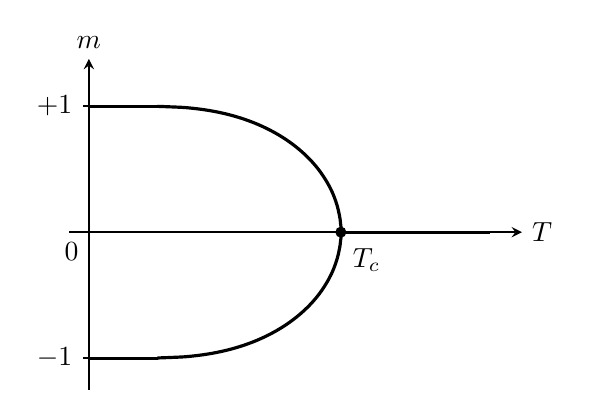
\begin{tikzpicture}[>=stealth, thick, scale=1.0]
  % Axes: T horizontal (0 to 5.4), m vertical (-2.0 to 2.2)
  % Tc at x = 3.2, m = +-1 at y = +-1.6
  \draw[->, line width=0.65pt] (-0.25, 0) -- (5.5, 0) node[right] {$T$};
  \draw[->, line width=0.65pt] (0, -2.0) -- (0, 2.2) node[above] {$m$};
  \node[below left] at (0, 0) {$0$};

  % Ticks for +-1 and Tc
  \draw[line width=0.55pt] (-0.07, 1.6) -- (0.07, 1.6);
  \node[left] at (-0.08, 1.6) {$+1$};
  \draw[line width=0.55pt] (-0.07, -1.6) -- (0.07, -1.6);
  \node[left] at (-0.08, -1.6) {$-1$};

  \draw[line width=0.55pt] (3.2, -0.07) -- (3.2, 0.07);
  \node[below right] at (3.22, -0.08) {$T_c$};

  % Parametric exact mean-field curve: m = tanh(m / t) => t = m / atanh(m)
  % where t = T / Tc in (0, 1), atanh(m) = 0.5*ln((1+m)/(1-m))
  % Upper stable branch (+m)
  \draw[line width=1.15pt, domain=0.02:0.999, samples=120, smooth]
    plot ({3.2 * \x / (0.5 * ln((1+\x)/(1-\x)))}, {1.6 * \x});
  \draw[line width=1.15pt] (0, 1.6) -- (0.88, 1.6);

  % Lower stable branch (-m)
  \draw[line width=1.15pt, domain=0.02:0.999, samples=120, smooth]
    plot ({3.2 * \x / (0.5 * ln((1+\x)/(1-\x)))}, {-1.6 * \x});
  \draw[line width=1.15pt] (0, -1.6) -- (0.88, -1.6);

  % m = 0 for T >= Tc (stable solid) and 0 < T < Tc (unstable dashed)
  \draw[line width=1.15pt] (3.2, 0) -- (5.1, 0);
  \draw[dashed, line width=0.75pt] (0, 0) -- (3.2, 0);

  \fill (3.2, 0) circle (2.0pt);
\end{tikzpicture}
\end{document}
